\section{Approximate Spanning Tree}\label{sec:ast}

\peace\/ uses a Minimum Spanning Tree (MST) based method for
clustering~\cite{rao-10}.  In this method, each read in a dataset is
deemed as a node in the MST.  The MST is constructed using Prims's
algorithm, with d2 scores serving as the edge weights.  Recollect
that, as discussed in Section~\ref{sec:background}, d2 scores tend to
zero for highly similar reads -- \ie\/ similar reads will be adjacent
or nearby branches in the MST.  Once an MST is constructed, clustering
is accomplished by cutting the MST at branches that are significantly
distant, based on a given clustering-threshold, currently set to 1.0
in \peace.  Note that this 1.0 is \emph{not} a normalized value but a
putative d2 score (with 10.0 corresponding to infinity) that indicates
sufficiently different reads.

The most time-consuming operation is the construction of MST.  The
most dominant issue is that MST construction is an $O(n^{2})$
algorithm (where $n$ is the number of reads), which is prohibitive for
large datasets~\cite{hazelhurst-11}.  MST construction results in
$n^{2}$ calls to d2-score computation, which in itself, is expensive
and requires few milliseconds.  Here, heuristics (than run in
microseconds) help by eliminating over 80\% of d2 comparisons.  The
proposed Prime Number based Heuristic (PNH) aims to help in this area
and is discussed in Section~\ref{sec:pnh}.  Nevertheless, the
remaining 20\% of d2 comparisons take substantial runtime.

The Approximate Spanning Tree (AST) aims to address the $O(n^{2})$
time complexity by rapidly adding nodes to the tree, thereby reducing
the time constants.  Note the AST does not change the asymptotic time
complexity of $O(n^{2})$ but rather aims to rapidly reduce $n$.  An
overview of the AST construction method is summarized in
Algorithm~\ref{alg:ast}.  The algorithm begins with a list of reads
(\q{estList}) and an arbitrarily chosen \q{root} read.  Next, given a
\q{root}, sufficiently similar reads are obtained via call to the
\q{getReads} method.  This method has an $O(n)$ time complexity and
uses heuristics to reduce the number of calls to the heavyweight
\q{d2} computation method.  Only reads that are below the specified
\q{ASTthresh} threshold are returned.

%% Bunch of shortcuts are defined below to streamline coding up the
%% AST agorithm below.

\definecolor{grey}{RGB}{175, 175, 175}
\definecolor{myBlue}{RGB}{0, 100, 200}

\SetNlSty{bfseries}{\color{grey}}{}
%\newcommand{\state}{\ArgSty{state}}
\SetKw{not}{!}
\SetKw{true}{true}
\newcommand{\ra} {\textrightarrow}
%\SetKw{false}{false}

%% The AST method
\SetKwBlock{AST}{begin AST(\ArgSty{estList}, \ArgSty{root}, \ArgSty{ASTthresh})}{end AST}

%% The getReads method
\SetKwBlock{getReads}{begin getReads(\ArgSty{estList}, \ArgSty{root}, \ArgSty{ASTthresh})}{end getReads}

% Style comments font and color
\newcommand\mycommfont[1]{\footnotesize\ttfamily\textcolor{myBlue}{#1}}
\SetCommentSty{mycommfont}

\begin{algorithm}[h]
  \AST{
    ast.add(root, 0) \tcp{d2 distance is 0}
    \While{\not estList.empty()}{
      \tcp{Get reads with d2 score \textless\/ ASTthresh}
      nearList = getReads(estList, root, ASTthresh)

      \tcp{Add all similar reads to AST}
      \ForEach{\textless est, d2score\textgreater\/ $\in$ nearList}{
        ast.add(root, est, d2score)
        
        estList.remove(est)
      }
      root = nearList.last().est
    }
    \Return{ast}
  }

  \getReads{
    nearList = \{\}
    
    \ForEach{est $\in$ estList}{
      \If{heuristicChain.shouldAnalyze(root, est)}{
        d2score = d2(root, est)
      
        \If{d2score \textless\/ ASTthresh}{
          nearList.add(\textless est, d2score\textgreater)
        }
      }
    }
    \Return{nearList}
  }
  \caption{Approximate Spanning Tree (AST)}\label{alg:ast}
\end{algorithm}


Unlike MST construction that adds only the most similar read, the AST
adds all of the similar reads, thereby rapidly reducing the number of
pending reads (\ie\/ $n$).  Reads are considered similar if their d2
distance is below a given AST-threshold value.  Similar to d2 scores,
the AST-threshold value is not normalized and this value cannot exceed
the clustering-threshold, which is currently set to 1.0.  The
AST-threshold value is a critical factor that influences the overall
performance.  The chart in Figure~\ref{fig:ast-thresh} illustrates the
impact of changing the threshold on a Haemagglutinin (HA) dataset with
\mytilde 65K reads.  Larger AST-thresholds allow more reads to be
added to the AST, thereby rapidly reducing $n$.  This results in fast
runtime but the resulting spanning tree drifts further away from the
MST.  In contrast, smaller threshold values result in a tree closer to
an MST -- \ie\/ AST-threshold of 0.0 produces an MST.  However,
smaller thresholds increase runtime with an $O(n^{2})$ time complexity
as illustrated by the inset chart in Figure~\ref{fig:ast-thresh}.

\begin{figure}
  \centerline{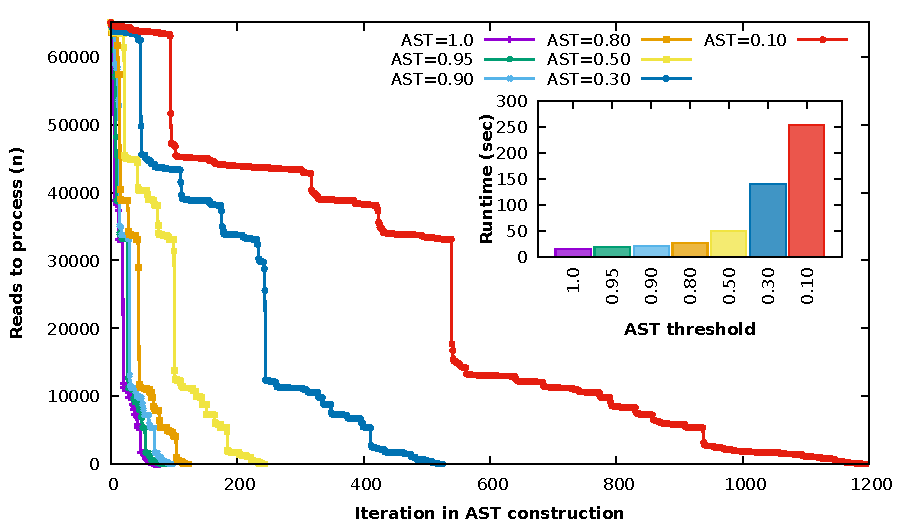
\includegraphics[width=\linewidth]{../charts/ha_1500_maxUse_convergence/maxUse_convergence.pdf}}
  \caption{Impact of AST threshold}\label{fig:ast-thresh}
\end{figure}

A comparison of MST and its corresponding AST is shown in
Figure~\ref{fig:mst-ast}.  The MST has been generated using 500 (for
readability) randomly chosen reads.  The AST has been generated with
an AST-threshold of 1.0 (\ie\/ \q{AST=1.0} in
Figure~\ref{fig:ast-thresh}).  The nodes in the tree have been
color-coded based on the clusters they were assigned.  The key feature
of interest is the structure of the two trees.  The MST has many
deeper branches because nodes are added one at a time.  On the other
hand, the AST has a much shallower structure with some nodes having a
very high degree.  The high degree nodes are the key in improving
performance as they enable many reads to be added to the AST thereby
rapidly reducing $n$ as illustrated by the curve for \q{AST=1.0} in
Figure~\ref{fig:ast-thresh}.

\begin{figure}[h]
  \begin{minipage}{\linewidth}
    \centerline{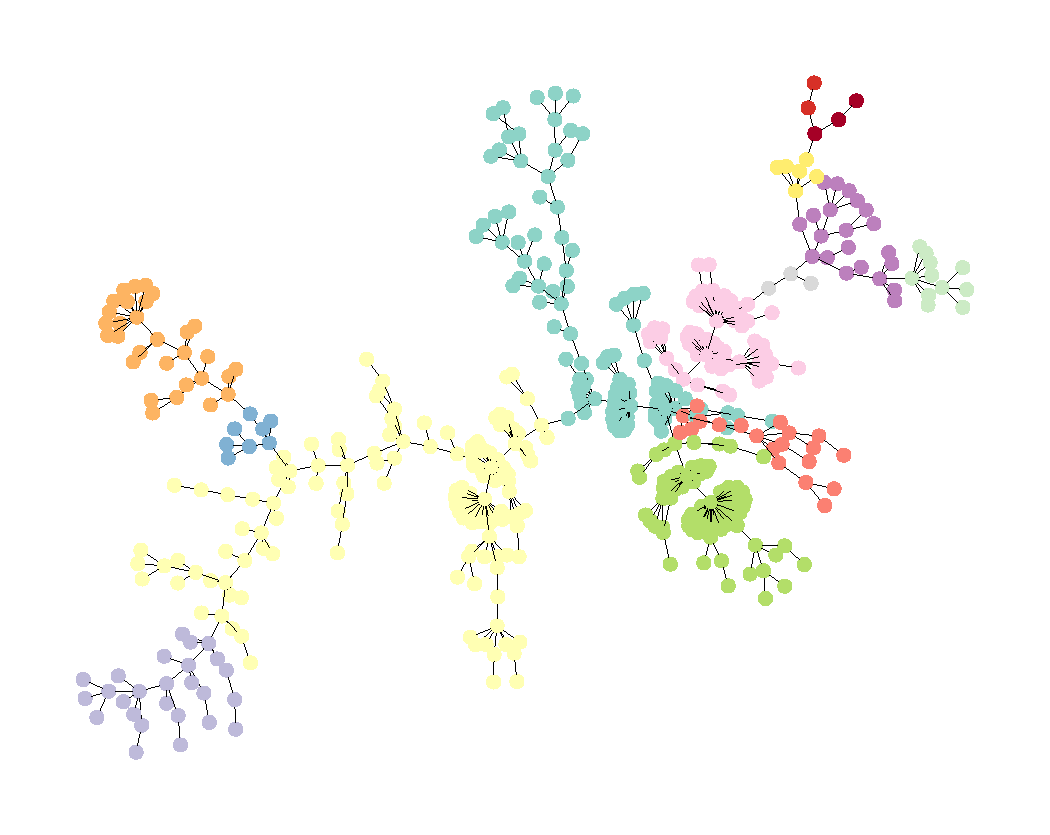
\includegraphics[width=\linewidth]{../charts/mst_vs_ast/ha_500_digraph.pdf}}
    \centerline{\footnotesize{(a) MST}}
  \end{minipage}
  
  \begin{minipage}{\linewidth}
    \centerline{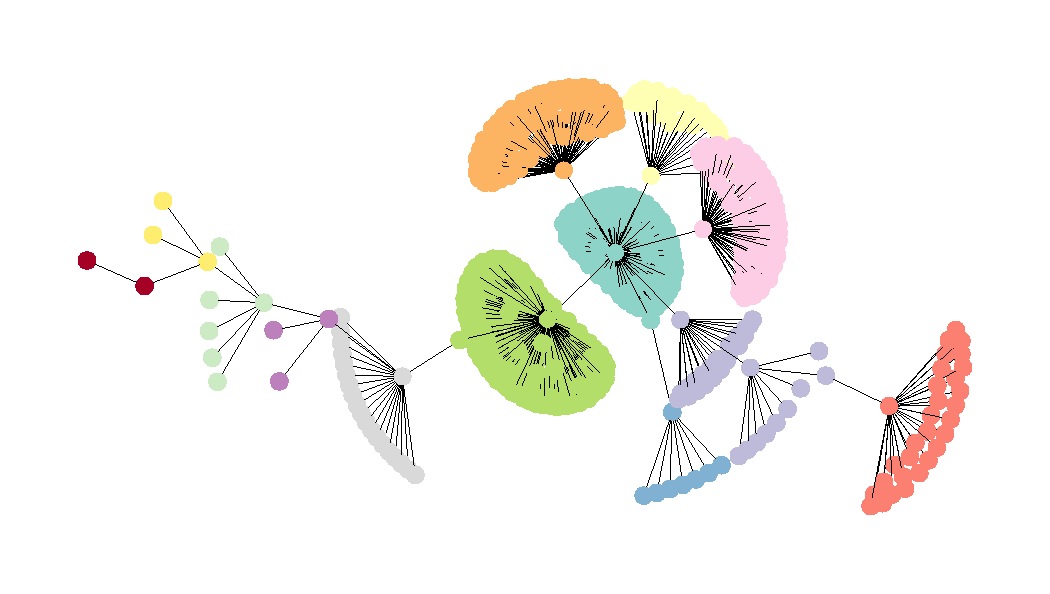
\includegraphics[width=\linewidth]{../charts/mst_vs_ast/ha_500_ast_digraph.pdf}}
    \centerline{\footnotesize{(b) AST}}
  \end{minipage}
  \caption{Comparison of MST and AST}\label{fig:mst-ast}
\end{figure}

The impact of varying the AST-threshold on the clustering quality is
illustrated by the charts in Figure~\ref{fig:ast-qual}.  As
illustrated by the NMI curve (see Section~\ref{sec:metrics} for
details on NMI), the quality of clustering degrades as the
AST-threshold is increased.  NMI degrades as the number of clusters
increases with increase in AST-threshold.  This is because in the AST
potentially shorter links are not captured.  This results in
additional edges to be cut causing more clusters to be generated.
However, as indicated by the chart, the purity of clustering does not
degrade -- \ie\/ the AST does not incorrectly cluster disparate reads
together.  The observation suggests that a cluster-merging operation
can optionally be used to reduce the number of clusters, if needed.

\begin{figure}[h]
  \centerline{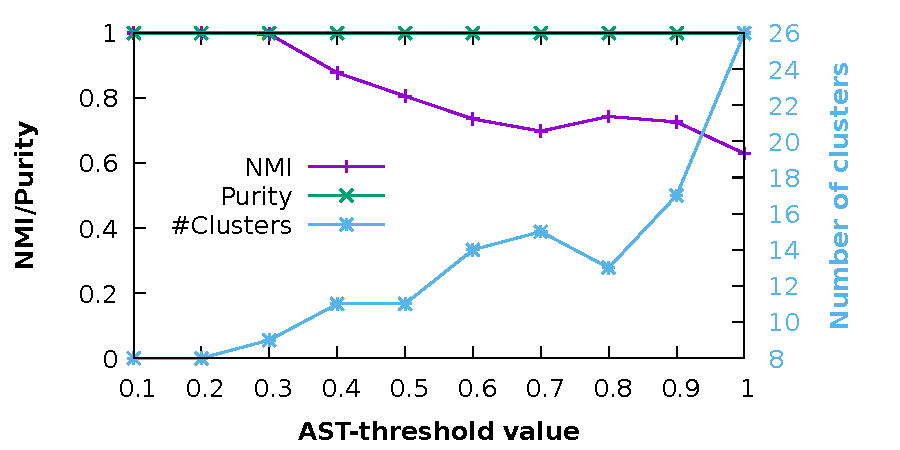
\includegraphics[width=\linewidth]{../charts/param_analysis/maxuse_quality.pdf}}
  \caption{Impact of AST-threshold}\label{fig:ast-qual}
\end{figure}
